\documentclass{scrartcl}

\usepackage{dsfont}
\usepackage{amsmath}
\usepackage{tikz}

\begin{document}

\title{Edge Basis and Transformation}

\maketitle

\section{The Basis}

For the edge basis we have the following properties, which fully determine
them:
\begin{subequations}
  \begin{enumerate}
  \item Each shape function $\psi_i$ is linear:
    \begin{equation}
      \psi^i(\mathbf x)=\mathrm A^i\mathbf x+\mathbf a^i
    \end{equation}
  \item Each shape function maps from $\mathds R^n$ to $\mathds R^n$, where
    $n$ is the dimension.
  \item For each shape function holds
    \begin{equation}
      \psi_i(\mathbf x)\cdot\mathbf t^j=\delta_{ij} \qquad
      \forall\mathbf x\in\Gamma^j,
    \end{equation}
    where $\Gamma^j$ denotes edge $j$ and $\mathbf t^j$ denotes a tangential
    unit vector to that edge.
  \end{enumerate}
\end{subequations}
We use the following numbering of edges and vertices:
\begin{center}
  \begin{tabular}[c]{c|c|c}
edge \# & vertex 0 \# & vertex 1 \# \\\hline
   0    &     0       &      1      \\
   1    &     0       &      2      \\
   2    &     1       &      2
 \end{tabular}
 \hspace{1cm}
 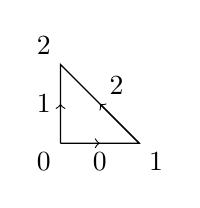
\begin{tikzpicture}[baseline={(.5,.5)}]
   \draw (0,0) node[below left] {0}
         -- node[below] {0}
         (1,0) node[below right] {1}
         -- node[above right] {2}
         (0,1) node[above left] {2}
         -- node[left] {1}
         (0,0);
   \draw[->] (0,0) -- (.5,0);
   \draw[->] (1,0) -- (.5,.5);
   \draw[->] (0,0) -- (0,.5);
 \end{tikzpicture}
\end{center}
From that follow the following definitions for the tangential unit vectors
$\mathbf t^i$ and edge lengthes $\ell^i$, where $\mathbf x^i$ are the
coordinates of vertex $i$:
\begin{subequations}
  \begin{align}
    \mathbf t^0&=(\mathbf x^1-\mathbf x^0)/\ell^0 &
         \ell^0&=||\mathbf x^1-\mathbf x^0||      \\
    \mathbf t^1&=(\mathbf x^2-\mathbf x^0)/\ell^1 &
         \ell^1&=||\mathbf x^2-\mathbf x^0||      \\
    \mathbf t^2&=(\mathbf x^2-\mathbf x^1)/\ell^2 &
         \ell^2&=||\mathbf x^2-\mathbf x^1||
  \end{align}
\end{subequations}
Evaluating the shape functions at the three vertices and taking the scalar
product with the two adjacent tangential vectors $\psi^i(\mathbf
x^k)\cdot\mathbf t^j=\delta_{ij}$ $\forall k\in\{j_0,j_1\}$ leaves us with
the following six conditions:
\begin{subequations}
  \begin{align}
    \label{cond:x0t0}
    \psi^i(\mathbf x^0)\cdot\mathbf t^0&=\delta_{i0} &&\Longrightarrow &
        (\mathrm A^i\mathbf x^0+\mathbf a^i)
        \cdot(\mathbf x^1-\mathbf x^0)&=\delta_{i0}\ell^0              \\
    \label{cond:x1t0}
    \psi^i(\mathbf x^1)\cdot\mathbf t^0&=\delta_{i0} &&\Longrightarrow &
        (\mathrm A^i\mathbf x^1+\mathbf a^i)
        \cdot(\mathbf x^1-\mathbf x^0)&=\delta_{i0}\ell^0              \\
    \label{cond:x1t2}
    \psi^i(\mathbf x^1)\cdot\mathbf t^2&=\delta_{i2} &&\Longrightarrow &
        (\mathrm A^i\mathbf x^1+\mathbf a^i)
        \cdot(\mathbf x^2-\mathbf x^1)&=\delta_{i2}\ell^2              \\
    \label{cond:x2t2}
    \psi^i(\mathbf x^2)\cdot\mathbf t^2&=\delta_{i2} &&\Longrightarrow &
        (\mathrm A^i\mathbf x^2+\mathbf a^i)
        \cdot(\mathbf x^2-\mathbf x^1)&=\delta_{i2}\ell^2              \\
    \label{cond:x2t1}
    \psi^i(\mathbf x^2)\cdot\mathbf t^1&=\delta_{i1} &&\Longrightarrow &
        (\mathrm A^i\mathbf x^2+\mathbf a^i)
        \cdot(\mathbf x^2-\mathbf x^0)&=\delta_{i1}\ell^1              \\
    \label{cond:x0t1}
    \psi^i(\mathbf x^0)\cdot\mathbf t^1&=\delta_{i1} &&\Longrightarrow &
        (\mathrm A^i\mathbf x^0+\mathbf a^i)
        \cdot(\mathbf x^2-\mathbf x^0)&=\delta_{i1}\ell^1
  \end{align}
\end{subequations}
By pairwise combination we can transform these conditions into
\begin{subequations}
  \begin{align}
    [\mathrm A^i(\mathbf x^1-\mathbf x^0)]
      \cdot(\mathbf x^1-\mathbf x^0)&=0 &&\Longleftrightarrow &
        (\mathrm A^i\mathbf t^0)\cdot\mathbf t^0&=0           \\
    [\mathrm A^i(\mathbf x^2-\mathbf x^0)]
      \cdot(\mathbf x^2-\mathbf x^0)&=0 &&\Longleftrightarrow &
        (\mathrm A^i\mathbf t^1)\cdot\mathbf t^1&=0           \\
    [\mathrm A^i(\mathbf x^2-\mathbf x^1)]
      \cdot(\mathbf x^2-\mathbf x^1)&=0 &&\Longleftrightarrow &
        (\mathrm A^i\mathbf t^2)\cdot\mathbf t^2&=0
  \end{align}
  and
  \begin{align}
    (\mathrm A^i\mathbf x^0+\mathbf a^i)\cdot(\mathbf x^2-\mathbf x^1)
        &=\delta_{i1}\ell^1-\delta_{i0}\ell^0 &&\Longleftrightarrow &
      (\mathrm A^i\mathbf x^0+\mathbf a^i)\cdot\mathbf t^2
        &=\frac{\delta_{i1}\ell^1-\delta_{i0}\ell^0}{\ell^2}        \\
    (\mathrm A^i\mathbf x^1+\mathbf a^i)\cdot(\mathbf x^2-\mathbf x^0)
        &=\delta_{i2}\ell^2+\delta_{i0}\ell^0 &&\Longleftrightarrow &
      (\mathrm A^i\mathbf x^1+\mathbf a^i)\cdot\mathbf t^1
        &=\frac{\delta_{i2}\ell^2+\delta_{i0}\ell^0}{\ell^1}         \\
    (\mathrm A^i\mathbf x^2+\mathbf a^i)\cdot(\mathbf x^1-\mathbf x^0)
        &=\delta_{i1}\ell^1-\delta_{i2}\ell^2 &&\Longleftrightarrow &
      (\mathrm A^i\mathbf x^2+\mathbf a^i)\cdot\mathbf t^0
        &=\frac{\delta_{i1}\ell^1-\delta_{i2}\ell^2}{\ell^0}
\end{align}
\end{subequations}
From the first three equations follows that the matrices $\mathrm A^i$ are
antisymmetric: Let $\mathrm A$ be a $2\times2$ matrix and $\mathbf t$ be a
vector with two entries.  Then the equation $(\mathrm A\mathbf t)\cdot\mathbf
t=0$ yields:
\begin{equation}
  (\mathbf t_0)^2\mathrm A_{00}
  +\mathbf t_0\mathbf t_1(\mathrm A_{01}+\mathrm A_{10})
  +(\mathbf t_1)^2\mathrm A_{11}=0
\end{equation}
This is certainly fulfilled for any antisymmetric matrix.  If we have three
vectors $\mathbf t^j$ which are mutually linearly independent, we have three
such equations, with which we can fix three of the four coefficients of
$\mathrm A$, and since antisymmetric matrices have only on independent
coefficient left and fulfill the above equation, $\mathrm A$ must be
antisymmetric.  Thus the three matrices $\mathrm A^i$ are antisymmetric:
\begin{equation}
  \mathrm A^i=\alpha^i\begin{pmatrix}0&1\\-1&0\end{pmatrix}
  =\alpha^i\mathds{\tilde1}
\end{equation}
The other three equations yield the following equation system:
\begin{equation}
  \begin{pmatrix}
    (\mathbf x^2-\mathbf x^1)\cdot\mathds{\tilde1}\mathbf x^0
            & \mathbf x^2_0-\mathbf x^1_0
                      & \mathbf x^2_1-\mathbf x^1_1  \\
    (\mathbf x^2-\mathbf x^0)\cdot\mathds{\tilde1}\mathbf x^1
            & \mathbf x^2_0-\mathbf x^0_0
                      & \mathbf x^2_1-\mathbf x^0_1  \\
    (\mathbf x^1-\mathbf x^0)\cdot\mathds{\tilde1}\mathbf x^2
            & \mathbf x^1_0-\mathbf x^0_0
                      & \mathbf x^1_1-\mathbf x^0_1
  \end{pmatrix}
  \begin{pmatrix}
    \alpha^i      \\
    \mathbf a^i_0 \\
    \mathbf a^i_1
  \end{pmatrix}
  =
  \begin{pmatrix}
    \delta_{i1}\ell^1-\delta_{i0}\ell^0 \\
    \delta_{i2}\ell^2+\delta_{i0}\ell^0 \\
    \delta_{i1}\ell^1-\delta_{i2}\ell^2
  \end{pmatrix}
\end{equation}

Mayhaps these will be useful later.

\section{Coordinate Transformation}

For transformation we use a mapping $\mathbf x=g(\mathbf{\hat x})$.  We say
that we map from {\em reference coordinates} $\mathbf{\hat x}$ into {\em world
  coordinates} $\mathbf x$.  Entities with the hat $\hat{\phantom x}$ are in
reference coordinates, entities without the hat are in world coordinates.  The
mapping $g$ is affine linear and can thus be written as
\begin{equation}
  g(\mathbf{\hat x})=\mathrm B\mathbf{\hat x}+\mathbf b
\end{equation}
The conversion of the vertex coordinates is simple:
\begin{equation}
  \mathbf x^i=\mathrm B\mathbf{\hat x}^i+\mathbf b
\end{equation}
The tangential vectors and edge lengthes are a bit more complicated:
\begin{subequations}
  \begin{align}
    \mathbf t^0&
      =\frac{\mathbf x^1-\mathbf x^0}{||\mathbf x^1-\mathbf x^0||}
      =\frac{\mathrm B(\mathbf{\hat x}^1-\mathbf{\hat x}^0)}
            {||\mathrm B(\mathbf{\hat x}^1-\mathbf{\hat x}^0)||}
      =\frac{\mathrm B\mathbf{\hat t}^0}{||\mathrm B\mathbf{\hat t}^0||}
    &  \ell^0&=||\mathbf x^1-\mathbf x^0||
              =||B(\mathbf{\hat x}^1-\mathbf{\hat x}^0)||               \\
    \mathbf t^1&
      =\frac{\mathbf x^2-\mathbf x^0}{||\mathbf x^2-\mathbf x^0||}
      =\frac{\mathrm B(\mathbf{\hat x}^2-\mathbf{\hat x}^0)}
            {||\mathrm B(\mathbf{\hat x}^2-\mathbf{\hat x}^0)||}
      =\frac{\mathrm B\mathbf{\hat t}^1}{||\mathrm B\mathbf{\hat t}^1||}
    &  \ell^1&=||\mathbf x^2-\mathbf x^0||
              =||B(\mathbf{\hat x}^2-\mathbf{\hat x}^0)||               \\
    \mathbf t^2&
      =\frac{\mathbf x^2-\mathbf x^1}{||\mathbf x^2-\mathbf x^1||}
      =\frac{\mathrm B(\mathbf{\hat x}^2-\mathbf{\hat x}^1)}
            {||\mathrm B(\mathbf{\hat x}^2-\mathbf{\hat x}^1)||}
      =\frac{\mathrm B\mathbf{\hat t}^2}{||\mathrm B\mathbf{\hat t}^2||}
    &  \ell^2&=||\mathbf x^2-\mathbf x^1||
              =||B(\mathbf{\hat x}^2-\mathbf{\hat x}^1)||
  \end{align}
\end{subequations}
If we require that $\hat\psi^i$ fullfills the same conditions in reference
coordinates as $\psi^i$ fullfills in world coordinates, what is the
transformation $\psi^i(g(\mathbf{\hat x}))=L(\hat\psi^i(\mathbf{\hat x}))$?
Let us assume that $L$ is linear and independent of $\mathbf x$ and
$\mathbf{\hat x}$:
\begin{equation}
  \mathbf y=L(\mathbf{\hat y})=\mathrm C\mathbf{\hat y}+\mathbf c
\end{equation}
How do $\mathrm C$ and $\mathbf c$ relate to $\mathrm B$ and $\mathbf b$?  

As special cases of $\mathbf y$ consider $\psi^i$.
\begin{gather}
  \psi^i(\mathbf x)=\mathrm A^i\mathbf x+\mathbf a^i
  =\mathrm C\hat\psi^i(\mathbf{\hat x})+\mathbf c
  =\mathrm C\mathrm{\hat A}^i\mathbf{\hat x}
      +\mathrm C\mathbf{\hat a}^i+\mathbf c\\
  \Downarrow\notag\\
  \mathrm A^i\mathrm B\mathbf{\hat x}+\mathrm A^i\mathbf b
      +\mathbf a^i
  =\mathrm C\mathrm{\hat A}^i\mathbf{\hat x}
      +\mathrm C\mathbf{\hat a}^i+\mathbf c
\end{gather}
Since this must hold for arbitrary $\mathbf{\hat x}$ it follows that
\begin{equation}
    \mathrm A^i\mathrm B=\mathrm C\mathrm{\hat A}^i
\end{equation}
and
\begin{equation}
  \mathrm A^i\mathbf b+\mathbf a^i=\mathrm C\mathbf{\hat a}^i+\mathbf c
\end{equation}
$\mathrm A^i$ and $\mathrm{\hat A}^i$ are antisymmetric:
\begin{align}
  \mathrm A^i&=\alpha^i\mathds{\tilde1}
  &\mathrm{\hat A}^i&=\hat\alpha^i\mathds{\tilde1}
\end{align}
$\mathds{\tilde1}$ is the ``antisymmetric unit matrix'' with the following
properties:
\begin{align}
  \mathds{\tilde1}&=\begin{pmatrix}0&1\\-1&0\end{pmatrix}     &
  \mathds{\tilde1}^{-1}&=-\mathds{\tilde1}=\mathds{\tilde1}^T  \\
  \mathds{\tilde1}^2&=-\mathds1                               &
  \mathds{\tilde1}\begin{pmatrix}a&b\\c&d\end{pmatrix}\mathds{\tilde1}
      &=\begin{pmatrix}-d&c\\b&-a\end{pmatrix}
       =-\begin{vmatrix}a&b\\c&d\end{vmatrix}
         \begin{pmatrix}a&b\\c&d\end{pmatrix}^{-T}
\end{align}
Thus follows
\begin{equation}
  \alpha^i\mathds{\tilde1}\mathrm B=\mathrm C\hat\alpha^i\mathds{\tilde1}
  \qquad\Longrightarrow\qquad
  \mathrm C=-\frac{\alpha^i}{\hat\alpha^i}\mathds{\tilde1}\mathrm
  B\mathds{\tilde1}
    =\frac{\alpha^i}{\hat\alpha^i}\det(\mathrm B)\mathrm B^{-T}
\end{equation}
So, $\mathrm C$ is a garbled and scaled version of $\mathrm B$.  Note that
\begin{equation}
  \frac{\alpha^0}{\hat\alpha^0}
  =\frac{\alpha^1}{\hat\alpha^1}
  =\frac{\alpha^2}{\hat\alpha^2}
\end{equation}
otherwise we would need a different $\mathrm C$ for each shape function.
We
have the three vertex coordinates times two directions in each coordinate to
evaluate $\psi^0$ and $\hat\psi^0$, that should give us six conditions with
which we should be able to fix the six coefficients of $\mathrm C$ and
$\mathbf c$ (ideally, $\mathbf c=0$).  OK, evaluating just one basis function
is probably not enough, since I already know what to expect there.  Instead, I
probably have to evaluate a function $\mathbf y(\mathbf x)$ ($\mathbf{\hat
  y}(\mathbf{\hat x})$) to learn whats going on.

Let
\begin{align}\label{ydef}
  \mathbf{\hat y}&=\sum_iy^i\hat\psi^i &&\text{and} &\mathbf y&=\sum_iy^i\psi^i
\end{align}
with the same coeffitients $y^i$.  Now we require
\begin{equation}
  \mathbf y(\mathbf x^i)=\mathrm C\mathbf{\hat y}(\mathbf{\hat x}^i)+\mathbf c.
\end{equation}
We will not test this with Cartesian components, but with the scalar product
of the function value with the tangential vectors:
\begin{equation}
  \mathbf{\hat y}(\mathbf{\hat x}^i)\cdot\mathbf{\hat t}^j
  =[\mathrm C\mathbf{\hat y}(\mathbf{\hat x}^i)]\cdot\mathbf t^j
  +\mathbf c\cdot\mathbf t^j  
\end{equation}
for edge $j$ adjacent to vertex $i$.  Inserting (\ref{ydef}) we get:
\begin{equation}
  \sum_ky^k\hat\psi^k(\mathbf{\hat x}^i)\cdot\mathbf{\hat t}^j
  =\sum_ky^k[\mathrm C\hat\psi^k(\mathbf{\hat x}^i)]\cdot\mathbf t^j
  +\mathbf c\cdot\mathbf t^j
\end{equation}
\begin{equation}
  \sum_ky^k\hat\psi^k(\mathbf{\hat x}^i)\cdot\mathbf{\hat t}^j
  =\sum_ky^k\psi^k(\mathbf x^i)\cdot\mathbf t^j
\end{equation}
For $\mathbf{\hat x}^i=\mathbf{\hat x}^0$ and $\mathbf{\hat t}^j=\mathbf{\hat
  t}^0$ we get
\begin{equation}
  \sum_ky^k\hat\psi^k(\mathbf{\hat x}^0)\cdot\mathbf{\hat t}^0
  =\left[\sum_ky^k\mathrm C\hat\psi^k(\mathbf{\hat x}^0)+\mathbf c\right]
    \cdot\frac{\mathrm B\mathbf{\hat t}^0}
              {||\mathrm B\mathbf{\hat t}^0||}
\end{equation}
Inserting (\ref{cond:x0t0}) on the left side and using the linearity of
$\hat\psi^k$ we get:
\begin{subequations}
  \begin{align}
    \mathbf{\hat x}^0,\mathbf{\hat t}^0&&
    y^0||\mathrm B\mathbf{\hat t}^0||
    &=\left[\sum_ky^k\mathrm C(\mathrm{\hat A}^k\mathbf{\hat x}^0
              +\mathbf{\hat a}^k)+\mathbf c\right]
      \cdot[\mathrm B\mathbf{\hat t}^0]\\
  \intertext{Similar for the other valid combinations:}
  \mathbf{\hat x}^1,\mathbf{\hat t}^0&&
    y^0||\mathrm B\mathbf{\hat t}^0||
    &=\left[\sum_ky^k\mathrm C(\mathrm{\hat A}^k\mathbf{\hat x}^1
              +\mathbf{\hat a}^k)+\mathbf c\right]
      \cdot[\mathrm B\mathbf{\hat t}^0]\\
  \mathbf{\hat x}^1,\mathbf{\hat t}^2&&
    y^2||\mathrm B\mathbf{\hat t}^2||
    &=\left[\sum_ky^k\mathrm C(\mathrm{\hat A}^k\mathbf{\hat x}^1
              +\mathbf{\hat a}^k)+\mathbf c\right]
      \cdot[\mathrm B\mathbf{\hat t}^2]\\
  \mathbf{\hat x}^2,\mathbf{\hat t}^2&&
    y^2||\mathrm B\mathbf{\hat t}^2||
    &=\left[\sum_ky^k\mathrm C(\mathrm{\hat A}^k\mathbf{\hat x}^2
              +\mathbf{\hat a}^k)+\mathbf c\right]
      \cdot[\mathrm B\mathbf{\hat t}^2]\\
  \mathbf{\hat x}^2,\mathbf{\hat t}^1&&
    y^1||\mathrm B\mathbf{\hat t}^1||
    &=\left[\sum_ky^k\mathrm C(\mathrm{\hat A}^k\mathbf{\hat x}^2
              +\mathbf{\hat a}^k)+\mathbf c\right]
      \cdot[\mathrm B\mathbf{\hat t}^1]\\
  \mathbf{\hat x}^0,\mathbf{\hat t}^1&&
    y^1||\mathrm B\mathbf{\hat t}^1||
    &=\left[\sum_ky^k\mathrm C(\mathrm{\hat A}^k\mathbf{\hat x}^0
              +\mathbf{\hat a}^k)+\mathbf c\right]
      \cdot[\mathrm B\mathbf{\hat t}^1]
  \end{align}
\end{subequations}
We substitute $\mathrm{\hat A}=\sum_ky^k\mathrm{\hat A}^k$ and $\mathbf{\hat a}=\sum_ky^k\mathbf{\hat a}^k$:
\begin{subequations}
  \begin{align}
    y^0||\mathrm B\mathbf{\hat t}^0||
    &=\left[\mathrm C(\mathrm{\hat A}\mathbf{\hat x}^0
              +\mathbf{\hat a})+\mathbf c\right]
      \cdot[\mathrm B\mathbf{\hat t}^0]\\
    y^0||\mathrm B\mathbf{\hat t}^0||
    &=\left[\mathrm C(\mathrm{\hat A}\mathbf{\hat x}^1
              +\mathbf{\hat a})+\mathbf c\right]
      \cdot[\mathrm B\mathbf{\hat t}^0]\\
    y^2||\mathrm B\mathbf{\hat t}^2||
    &=\left[\mathrm C(\mathrm{\hat A}\mathbf{\hat x}^1
              +\mathbf{\hat a})+\mathbf c\right]
      \cdot[\mathrm B\mathbf{\hat t}^2]\\
    y^2||\mathrm B\mathbf{\hat t}^2||
    &=\left[\mathrm C(\mathrm{\hat A}\mathbf{\hat x}^2
              +\mathbf{\hat a})+\mathbf c\right]
      \cdot[\mathrm B\mathbf{\hat t}^2]\\
    y^1||\mathrm B\mathbf{\hat t}^1||
    &=\left[\mathrm C(\mathrm{\hat A}\mathbf{\hat x}^2
              +\mathbf{\hat a})+\mathbf c\right]
      \cdot[\mathrm B\mathbf{\hat t}^1]\\
    y^1||\mathrm B\mathbf{\hat t}^1||
    &=\left[\mathrm C(\mathrm{\hat A}\mathbf{\hat x}^0
              +\mathbf{\hat a})+\mathbf c\right]
      \cdot[\mathrm B\mathbf{\hat t}^1]
  \end{align}
\end{subequations}
By pairwise combination we get the following:
\begin{subequations}
  \begin{align}
    0&=[\mathrm C\mathrm{\hat A}\mathbf{\hat t}^0]
      \cdot[\mathrm B\mathbf{\hat t}^0]\\
    0&=[\mathrm C\mathrm{\hat A}\mathbf{\hat t}^2]
      \cdot[\mathrm B\mathbf{\hat t}^2]\\
    0&=[\mathrm C\mathrm{\hat A}\mathbf{\hat t}^1]
      \cdot[\mathrm B\mathbf{\hat t}^1]
  \end{align}
\end{subequations}

\end{document}

%%% Local Variables: 
%%% mode: latex
%%% mode: TeX-PDF
%%% mode: auto-fill
%%% TeX-master: t
%%% mode: flyspell
%%% ispell-local-dictionary: "american"
%%% End: 
